\documentclass[11pt,a4paper]{article}

\usepackage[utf8]{inputenc}
\usepackage[spanish]{babel}
\usepackage{amsmath}
\usepackage{amsfonts}
\usepackage{amssymb}
\usepackage{url}
\usepackage[colorlinks,linktocpage=true,citecolor=blue,linkcolor=blue]{hyperref}
\usepackage{booktabs}
\usepackage{graphicx,geometry}
\usepackage{caption}
\usepackage{verbatim,moreverb}

\usepackage{listings}
\lstset{
	frame=tb,
    framerule=0pt,
    aboveskip=3mm,
    belowskip=3mm,
    framextopmargin=3pt,
    framexbottommargin=3pt,
    %framexleftmargin=0.2cm,
    framesep=0pt,
    rulesep=.4pt,
    backgroundcolor=\color{gray97},
    rulesepcolor=\color{black},
    stringstyle=\color{mauve},
    showstringspaces = false,
    basicstyle=\footnotesize\ttfamily,
    commentstyle=\color{dkgreen},
    keywordstyle=\color{blue},
    numbers=left,
    numbersep=-6.5pt,
    numberstyle=\tiny\color{gray},
    numberfirstline = false,
    breaklines=true,
    morekeywords={*,...}
   }

\usepackage{xcolor}
\definecolor{gray97}{gray}{.97}
\definecolor{gray75}{gray}{.75}
\definecolor{gray45}{gray}{.45}
\definecolor{mauve}{rgb}{0.58,0,0.82}
\definecolor{dkgreen}{rgb}{0,0.6,0}

\author{Marcos Rial Docampo}
\title{Técnicas de Análisis Cuantitativas y Cualitativas\\Resolución del ejercicio de evaluación 2}
\date{\small{\today}}

\begin{document}
\maketitle

En este ejercicio de evaluación se nos presentan datos de superficie agrícola abandonada, densidad de población y altitud media de una serie de 50 observaciones tomadas en otros tantos municipios gallegos. Se destaca la importancia que tiene la densidad de población o la elevación sobre los cambios de uso de suelo que afectan a superficie agrícola.

En los gráficos de la figura \ref{fig:graficas} se presenta la relación existente entre el abandono de la superficie agrícola y las otras dos variables: elevación y densidad de población. A primera vista podemos observar como aparentemente la relación entre el abandono y la densidad de población no ofrece indicios de correlación entre ambas. Lo que no ocurre con la segunda relación entre el abandono y la elevación, donde sí puede haber correlación. Pero esta es una valoración a priori solo observando el aspecto de las relaciones en una gráfica. Podría ser que alguna de las variables necesitara ser transformada para que en la gráfica se ofreciera una visión más fidedigna, pero no se ve necesario.

\begin{figure}
	\centering
	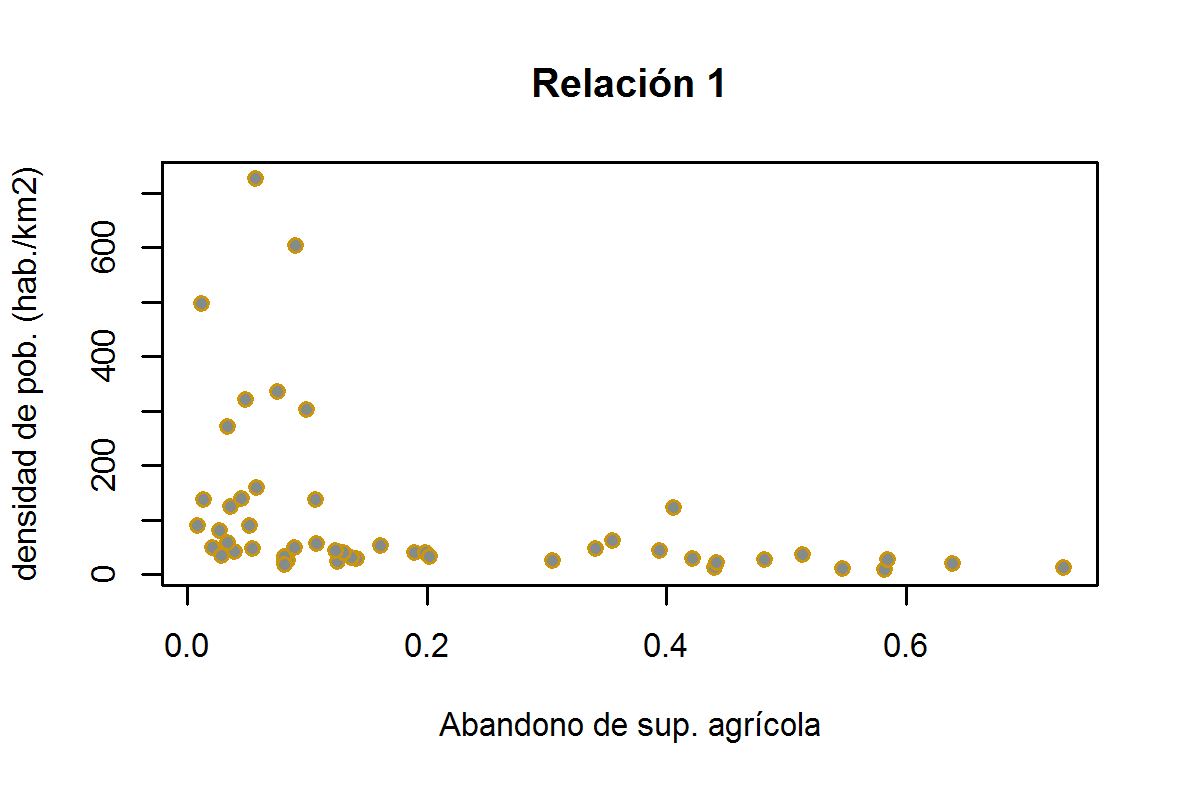
\includegraphics{./R/Graficos/Relacion1.png}
	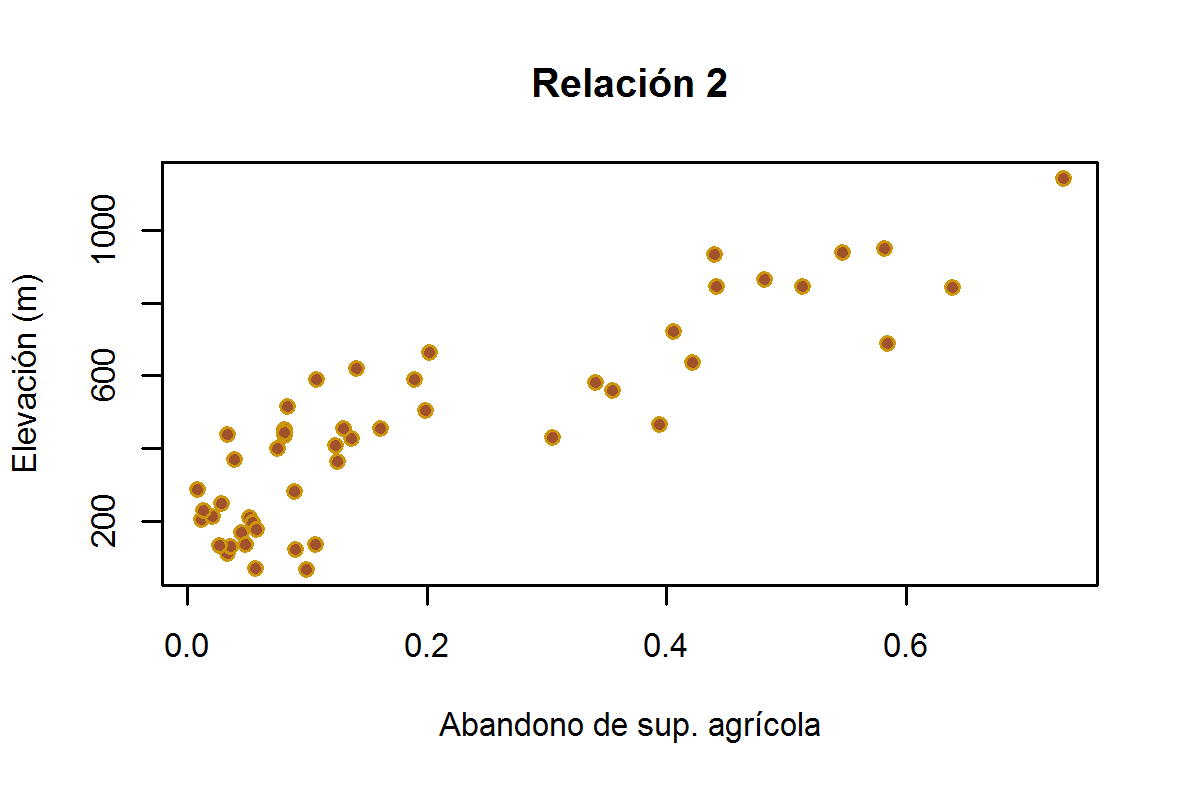
\includegraphics{./R/Graficos/Relacion2.png}
	\captionsetup{font={footnotesize,it}}
	\caption{Relación entre el abandono de superficie agrícola y las variables densidad de población y elevación.}
	\label{fig:graficas}
\end{figure}

Comprobamos la existencia de correlación entre las variables abandono y elevación y densidad de población. Partimos de la hipótesis nula (H$_0$) de que no existe correlación entre las dos variables estudiadas en cada caso. Para ello empleamos el comando de R \textit{cor.test()} como se muestra en la figura \ref{fig:cor.test}. Vemos en la figura \ref{fig:res.corr} que los resultados nos arrojan una alta correlación entre la variable abandono y la de elevación (coeficiente de Pearson de 0,8718). Mientras que para la otra relación, entre el abandono y la densidad de población, la correlación no existe (coeficiente de Pearson de -0,5379). Se confirma lo expuesto en el párrafo anterior.

\begin{figure}
\centering
\begin{lstlisting}[language = R]
  # Estudio de correlacion entre variables
  # H0 = las variables no estan correlacionadas
  # Abandono vs densidad de poblacion
  cor.test(datos$abandon.uaa, datos$pop.dens, alternative = "greater",
           method = "pearson", conf.level = 0.95)
  # Abandono vs elevacion
  cor.test(datos$abandon.uaa, datos$elevation, alternative = "greater",
           method = "pearson", conf.level = 0.95)
\end{lstlisting}
\captionsetup{font={footnotesize,it}}
\caption{Empleo del comando \textit{cor.test} con el método de Pearson y nivel de confianza al 95\%.}
\label{fig:cor.test}
\end{figure}

\begin{figure}
\centering
\begin{boxedverbatim}
    Pearson's product-moment correlation

data:  datos$abandon.uaa and datos$pop.dens
t = -2.6908, df = 48, p-value = 0.9951
alternative hypothesis: true correlation is greater than 0
95 percent confidence interval:
 -0.5505354  1.0000000
sample estimates:
       cor 
-0.3620322
\end{boxedverbatim}

\begin{boxedverbatim}
    Pearson's product-moment correlation

data:  datos$abandon.uaa and datos$elevation
t = 12.328, df = 48, p-value < 2.2e-16
alternative hypothesis: true correlation is greater than 0
95 percent confidence interval:
 0.8006674 1.0000000
sample estimates:
       cor 
0.8717672 
\end{boxedverbatim}
\captionsetup{font={footnotesize,it}}
\caption{Resultados del test de correlación.}
\label{fig:res.corr}
\end{figure}

Podemos obtener un modelo de regresión lineal múltiple entre variables obteniendo de este el plano de regresión:
\begin{equation}
y=-0.1375+0.0002x_{1}+0.0007x_{2}
\label{eq:regre.multi}
\end{equation}
\noindent siendo \textit{y} la variable abandono y $x_{1}$ y $x_2$ las variables densidad de población y elevación.

De dicho modelo de regresión múltiple extraemos la información que nos permitirá saber que variable es significativa y cual no, en el caso de haberlas, respecto de la variable abandono. Observamos los coeficientes de regresión ofrecidos de el cuadro \ref{tab:coef.multi} donde vemos que existe una fuerte relación del abandono con la variable elevación, mientras que con la variable densidad de población es menor.

\begin{table}
\centering
\begin{tabular}{ccccc}
\toprule[0.4mm]
& Estimate & Std. Error & t value & Pr$(>|t|)$\\
\midrule
(Intercept) & -1.375e-01 & 3.732e-02 & -3.684 & 0.000592\\
pop.dens & 1.967e-04 & 1.071e-04 & 1.837 & 0.072527\\
elevation & 6.987e-04 & 6.005e-05 & 11.635 & 1.94e-15\\
\bottomrule[0.4mm]
\end{tabular}
\captionsetup{font={footnotesize,it}}
\caption{Resultados del análisis de significación de la regresión múltiple.}
\label{tab:coef.multi}
\end{table}

Analizamos los supuestos de partida (figura .........).

Ahora, una vez aplicado un modelo de regresión múltiple y extraída la información obtendremos la recta de regresión entre la variable abandono y elevación (puesto que es la única relación que presenta correlación) obtenemos la gráfica de la figura \ref{fig:lm2} y observamos gracias a invocar el valor ``modelo2'', creado para aplicar la función de regresión lineal \textit{lm()} como en el caso anterior, que devuelve los coeficientes de significación que nos permiten obtener la recta de regresión:
\begin{equation}
y=-0.0896+0.0006x
\label{eq:regre.elev}
\end{equation}
\noindent siendo \textit{y} la variable abandono y \textit{x} la variable elevación.

\begin{figure}
	\centering
	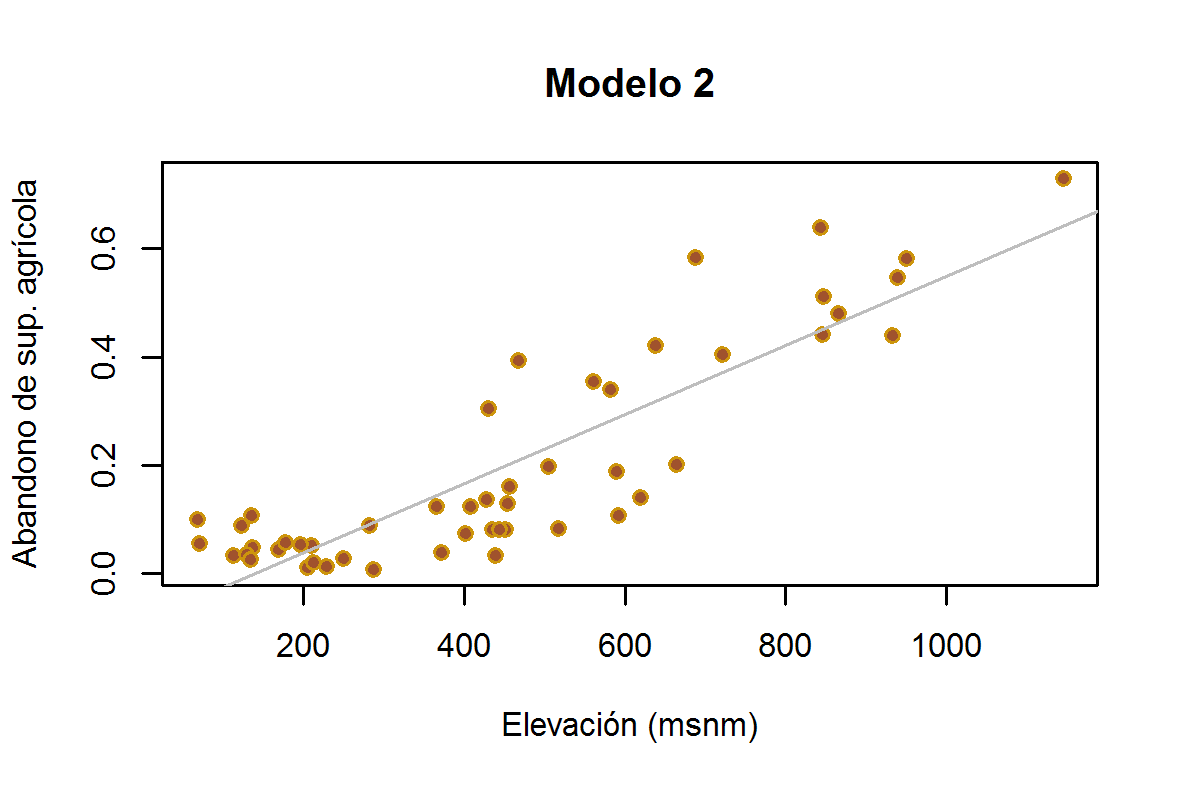
\includegraphics{./R/Graficos/Modelo2.png}
	\captionsetup{font={footnotesize,it}}
	\caption{Modelo de regresión lineal para la relación entre abandono y elevación.}
	\label{fig:lm2}
\end{figure}

\end{document}